% BEGIN LICENSE BLOCK
% Version: CMPL 1.1
%
% The contents of this file are subject to the Cisco-style Mozilla Public
% License Version 1.1 (the "License"); you may not use this file except
% in compliance with the License.  You may obtain a copy of the License
% at www.eclipse-clp.org/license.
% 
% Software distributed under the License is distributed on an "AS IS"
% basis, WITHOUT WARRANTY OF ANY KIND, either express or implied.  See
% the License for the specific language governing rights and limitations
% under the License. 
% 
% The Original Code is  The ECLiPSe Constraint Logic Programming System. 
% The Initial Developer of the Original Code is  Cisco Systems, Inc. 
% Portions created by the Initial Developer are
% Copyright (C) 2006 Cisco Systems, Inc.  All Rights Reserved.
% 
% Contributor(s): 
% 
% END LICENSE BLOCK
%
% $Id: modelling.tex,v 1.1.1.1 2006/09/23 01:49:52 snovello Exp $
%

%----------------------------------------------------------------------
\chapter{Problem Modelling}
%HEVEA\cutdef[1]{section}
%----------------------------------------------------------------------


%----------------------------------------------------------------------
\section{Constraint Logic Programming}
%----------------------------------------------------------------------

\index{Constraint Logic Programming}
\index{modelling}
One of the main ambitions of Constraint Programming is the
separation of Modelling, Algorithms and Search.
This is best characterised by two pseudo-equations.
\index{Kowalski}
The first one is paraphrased from Kowalski \cite{kowalski79}
\begin{quote}\begin{verbatim}
Solution = Logic + Control
\end{verbatim}\end{quote}
and states that we intend to solve a problem by
giving a logical, declarative description of the problem and
adding control information that enables a computer to deduce a solution.

\index{combinatorial problems}
The second equation
\begin{quote}\begin{verbatim}
Control = Reasoning + Search
\end{verbatim}\end{quote}
is motivated by a fundamental difficulty we face when dealing with
combinatorial problems: we do not have efficient algorithms
for finding solutions, we have to resort to a combination of
reasoning (via efficient algorithms) and (inefficient) search.

We can consider every constraint program as an exercise in
combining the 3 ingredients:
\begin{itemize}
\item {\bf Logic} -  The design of a declarative {\em Model} of the problem.
\item {\bf Reasoning} - The choice of clever {\em Constraint Propagation}
    algorithms that reduce the need for search.
\item {\bf Search} - The choice of search {\em strategies and heuristics} for
    finding solutions quickly.
\end{itemize}
In this chapter we will focus on the first issue, {\bf Problem Modelling},
and how it is supported by \eclipse{}.


%----------------------------------------------------------------------
\section{Issues in Problem Modelling}
%----------------------------------------------------------------------

A good formalism for problem modelling should fulfil the following criteria:
\begin{itemize}
\item {\bf Expressive power} - 
        Can we write a formal model of the real world problem?
\item {\bf Clarity for humans} - 
        How easily can the model be written, read, understood or modified?
\item {\bf Solvability for computers} - 
        Are there good known methods to solve it?
\end{itemize}
%In \eclipse{}, we model problems using a high-level logic-based language.
Higher-level models are typically
closer to the user and close to the problem and therefore
easier to understand and to trust,
easier to debug and to verify,
and easier to modify when customers change their mind.
On the other hand, it is not necessarily easy to see how they can be
solved, because high-level models contain
high-level notions (e.g.\ sets, tasks) and
heterogeneous constraints.

The constraint programming approach also addresses one of the classical
sources of error in application development with
traditional programming languages: the transition from a
{\em formal description}
of the problem to the {\em final program} that solves it.
%\begin{itemize}
%\item  Informal specification, which leads to a
%\item  Formal description, which leads to a
%\item  Program
%\end{itemize}
The question is: Can the final program be trusted?
The Constraint (Logic) Programming solution is to
\begin{itemize}
\item   Keep the initial formal model as part of the final program
\item   Enhance rather than rewrite
\end{itemize}
The process of enhancing the initial formal model involves for example
\begin{itemize}
\item Adding control annotations, e.g.
    algorithmic information or heuristic information.
\item Transformation:
    Mapping high-level (problem) constraints into
    low-level (solver) constraints,
    possibly exploiting multiple, redundant mappings.
\end{itemize}
There are many other approaches to problem modelling software.
The following is a brief comparison:
\begin{description}
\item[Formal specification languages (e.g. Z, VDM)]
    \index{specification languages}
    More expressive power than ECLiPSe, but not executable
\item[Mathematical modelling languages (e.g. OPL, AMPL)]
    \index{mathematical modelling languages}
    Similar to ECLiPSe, but usually limited expressive power,
    e.g.\ fixed set of constraints.
\item[Mainstream programming languages (e.g. C++ plus solver library)]
    \index{C++}
    Variables and constraints are "aliens" in the language.
    Specification is mixed with procedural control.
\item[Other CLP/high-level languages (e.g. CHIP)]
    \index{CHIP}
    Most similar to ECLiPSe. Less support for hybrid problem solving.
    Harder to define new constraints.
\end{description}



\section{Modelling with CLP and \eclipse{}}

When modelling problems with constraints, the basic idea is to set up
a network of variables and constraints. Figure \ref{figconsnet} shows
such a constraint network.
\begin{figure}
\begin{center}
\resizebox{0.7\textwidth}{!}{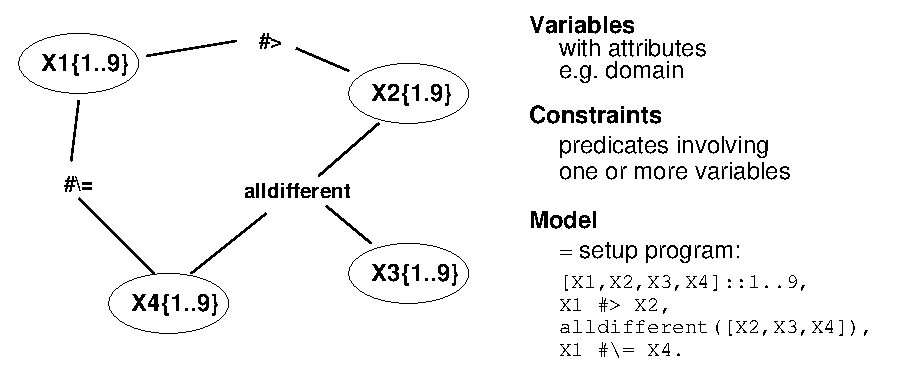
\includegraphics{consnet.eps}}
\end{center}
\caption{A Constraint Network}
\label{figconsnet}
\end{figure}
It can be seen that the Constraint Logic Programming (CLP) formulation
\begin{itemize}
\item is a natural declarative description of the constraint network
\item can serve as a program to set up the constraint network
\end{itemize}
\ignore{
The following properties make CLP langauges like
\eclipse[] suited as a modelling language:
\begin{description}
\item[Simple language]
    Logical variables,
    logical connectives (and, or, implication),
    predicates (relations, constraints),
    a single compound data type (structure),
    symbolic equality (unification)
\item[Logical reading]
        {\tt Program = Logic + Control}
\item[Flexible syntax]
        {\tt TaskA uses ResourceB}
\item[Symbolic and meta-programming capability]
        Easy to add domain-specific language features
\end{description}
}
The main \eclipse{} language constructs used in modelling are
\begin{description}
\item[Built-in constraints]\ \\
    \verb?X #> Y?
\item[Abstraction]\ \\
    \verb?before(task(Si,Di), task(Sj,Dj)) :- Si+Di #<= Sj.?
\item[Conjunction]\ \\
    \verb?between(X,Y,Z) :- X #< Y, Y #< Z.?
\item[Disjunction (but see below)]\ \\
    \verb?neighbour(X,Y) :- ( X #= Y+1 ; Y #= X+1 ).?
\item[Iteration]\ \\
    \verb?not_among(X, L) :- ( foreach(Y,L),param(X) do X #\= Y ).?
\item[Recursion]\ \\
    \verb?not_among(X, []).?\\
    \verb?not_among(X, [Y|Ys]) :- X #\= Y, not_among(X, Ys).?
\end{description}


%----------------------------------------------------------------------
\section{Same Problem - Different Model}
%----------------------------------------------------------------------

There are often many ways of modelling a problem.
Consider the famous "SEND + MORE = MONEY" example:
\begin{code}
sendmore(Digits) :-
    Digits = [S,E,N,D,M,O,R,Y],
    Digits :: [0..9],
    alldifferent(Digits),
    S #\verb.\.= 0, M #\verb.\.= 0,
                 1000*S + 100*E + 10*N + D
               + 1000*M + 100*O + 10*R + E
    #= 10000*M + 1000*O + 100*N + 10*E + Y.
\end{code}
An alternative model is based on the classical decimal addition algorithm with
carries:
\begin{code}
sendmore(Digits) :-
    Digits = [S,E,N,D,M,O,R,Y],
    Digits :: [0..9],
    Carries = [C1,C2,C3,C4],
    Carries :: [0..1],
    alldifferent(Digits),
    S #\verb.\.= 0,
    M #\verb.\.= 0,
    C1         #= M,
    C2 + S + M #= O + 10*C1,
    C3 + E + O #= N + 10*C2,
    C4 + N + R #= E + 10*C3,
         D + E #= Y + 10*C4.
\end{code}
Both models work fine, but obviously involve different variables and
constraints. Even though high-level models reduce the need for finding
sophisticated encodings of problems, finding good models still requires
substantial expertise and experience.

\ignore{
Abstraction

:- lib(ria).                            % Using interval library

farm(F) :-
        [A,B,C] :: 0.0..inf,            % The 3 sides of the lake
        triangle_area(A, B, C, 7),      % The lake area is 7

        [F,FA,FB,FC] :: 1..inf,         % The square areas are integral
        square_area(A, FA),
        square_area(B, FB),
        square_area(C, FC),
        F *= FA+FB+FC,

        FA *>= FB, FB *>= FC.           % Avoid symmetric solutions

triangle_area(A, B, C, Area) :-
        S *>= 0,
        S *= (A+B+C)/2,
        Area *= sqrt(S*(S-A)*(S-B)*(S-C)).

square_area(A, Area) :-
        Area *= sqr(A).
}


\ignore{
\subsection{Using Data Structures}

Structures
Task = task(plumbing, S, 3, R, _)
Task = task with [duration:3, resource:R, start:S, name:plumbing]
Lists
Digits = [S,E,N,D,M,O,R,Y]
length(VarList, 100)
Arrays
dim(ChessBoard, [8,8])
VarArray =.. [_|VarList]

In ECLiPSe, lists and arrays are just special structures!
}



\section{Rules for Modelling Code}

In CLP, the declarative model is at the same time the constraint setup code.
This code should therefore be deterministic and terminating, so:
\begin{description}
\item[Careful with disjunctions]
    Don't leave choice-points (alternatives for backtracking).
    Choices should be deferred until search phase.
\item[Use only simple conditionals]
    Conditions in \verb=(...->...;...)= must be true or false at modelling time!
\item[Use only structural recursion and loops]
    Termination conditions must be know at modelling time!
\end{description}

\subsection{Disjunctions}

Disjunctions in the model should be avoided. Assume that a naive
model would contain the following disjunction:
\begin{code}
% DO NOT USE THIS IN A MODEL
no_overlap(S1,D1,S2,D2) :- S1 #>= S2 + D2.
no_overlap(S1,D1,S2,D2) :- S2 #>= S1 + D1.
\end{code}
There are two basic ways of treating the disjunction:
\begin{itemize}
\item Deferring the choice until the search phase by introducing a
        decision variable.
\item Changing the behaviour of the disjunction so it becomes a constraint
        (see also \ref{chapimpl} and \ref{chappropiachr}).
\end{itemize}
In the example, we can introduce a boolean variable \verb.B{0,1}. which represents
the choice.
The actual choice can be then be taken in search code by choosing a
value for the variable. The model code must then be changed to observe
the decision variable, either using the delay facility of \eclipse{}:
\begin{code}
delay no_overlap(S1,D1,S2,D2,B) if var(B).
no_overlap(S1,D1,S2,D2,0) :- S1 #>= S2 + D2.
no_overlap(S1,D1,S2,D2,1) :- S2 #>= S1 + D1.
\end{code}
or using an arithmetic encoding like in
\begin{code}
no_overlap(S1,D1,S2,D2,B) :-
        B :: 0..1, 
        S1 +     B*1000 #>= S2 + D2,
        S2 + (1-B)*1000 #>= S1 + D1.
\end{code}
The alternative of turning the disjunction into a proper constraint is
achieved most easily using {\em propia}'s infer-annotation
(see \ref{chappropiachr}). The original formulation of neighbour/2
is kept but it is used as follows:
\begin{code}
    ..., no_overlap(S1,D2,S2,D2) infers most, ...
\end{code}


\subsection{Conditionals}

Similar considerations apply to conditionals where the condition is not
decidable at constraint setup time. For example, suppose we want to
impose a no-overlap constraint only if two tasks share the same resource.
The following code is currently not safe in ECLiPSe:
\begin{code}
nos(Res1, Res2, Start1, Dur1, Start2, Dur2) :-
    ( Res1 #= Res2 ->           % WRONG!!!
        no_overlap(Start1, Dur1, Start2, Dur2)
    ;
        true
    )
\end{code}
The reason is that (at constraint setup time) Res1 and Res2 will most
likely be still uninstantiated. Therefore, the condition will in general
delay (rather than succeed or fail), but the conditional construct
will erroneously take this for a success and take the first alternative.

Again, this can be handled using delay
\begin{code}
delay nos(Res1, Res2, _, _, _, _) if nonground([Res1,Res2]).
nos(Res1, Res2, Start1, Dur1, Start2, Dur2) :-
    ( Res1 == Res2 ->
        no_overlap(Start1, Dur1, Start2, Dur2)
    ;
        true
    ).
\end{code}
It might also be possible to compute a boolean variable indicating the
truth of the condition. This is particularly easy when a reified
constraint can be used to express the condition, like in this case:
\begin{code}
nos(Res1, Res2, Start1, Dur1, Start2, Dur2) :-
    #=(Res1, Res2, Share),
    cond_no_overlap(Start1, Dur1, Start2, Dur2, Share).

delay cond_no_overlap(_,_,_,_,Share) if var(Share).
cond_no_overlap(Start1, Dur1, Start2, Dur2, Share) :-
    ( Share == 1 ->
        no_overlap(Start1, Dur1, Start2, Dur2)
    ;
        true
    ).
\end{code}


\section{Symmetries}

Consider the following puzzle, where numbers from 1 to 19 have to be arranged
in a hexagonal shape such that every diagonal sums up to 38:
\begin{code}
puzzle(Pattern) :-
        Pattern = [
                   A,B,C,
                  D,E,F,G,
                 H,I,J,K,L,
                  M,N,O,P,
                   Q,R,S
                  ],
        Pattern :: 1 .. 19,

        % Problem constraints
        alldifferent(Pattern),
          A+B+C #= 38,     A+D+H #= 38,     H+M+Q #= 38,
         D+E+F+G #= 38,   B+E+I+M #= 38,   D+I+N+R #= 38,
        H+I+J+K+L #= 38, C+F+J+N+Q #= 38, A+E+J+O+S #= 38,
         M+N+O+P #= 38,   G+K+O+R #= 38,   B+F+K+P #= 38,
          Q+R+S #= 38,     L+P+S #= 38,     C+G+L #= 38,
        ...
\end{code}
In this formulation, the problem has 12 solutions, but it turns out they
are just rotated and mirrored variants of each other.
Removal of symmetries is still an area of active research, but a simple
method is applicable in situations like this one.
One can add constraints which require the solution to have certain
additional properties, and so exclude many of the symmetric solutions:
\begin{code}
        ...,
        % Optional anti-symmetry constraints
        % Forbid rotated solutions: require A to be the smallest corner
        A #< C, A #< H, A #< L, A #< S, A #< Q,
        % Forbid solutions mirrored on the A-S diagonal
        C #< H.
\end{code}

%HEVEA\cutend
